\documentclass[12pt, a4paper]{article}
\usepackage{graphicx} 
\usepackage{geometry}
\geometry{a4paper, margin=1in}
\usepackage{tikz}
\usetikzlibrary{calc}
\usepackage{hyperref} 
\usepackage{color}
\usepackage{array} % For centering content in table cells
\usepackage{lipsum} % For placeholder text
\usepackage{listings}
\usepackage{xcolor}

% Define custom colors for better readability
\definecolor{codegray}{rgb}{0.5, 0.5, 0.5}
\definecolor{codegreen}{rgb}{0, 0.6, 0}
\definecolor{codeblue}{rgb}{0.2, 0.2, 0.8}
\definecolor{codered}{rgb}{0.7, 0.1, 0.1}
\definecolor{background}{rgb}{0.95, 0.95, 0.92}

\lstset{
    language=C,                            % Code language
    backgroundcolor=\color{background},    % Set background color
    basicstyle=\ttfamily\small,            % Font style and size
    keywordstyle=\color{codeblue}\bfseries,% Keyword style
    stringstyle=\color{codered},           % String style
    commentstyle=\color{codegreen}\itshape,% Comment style
    morecomment=[l][\color{magenta}]{\#},  % Special comment style
    numbers=left,                          % Line numbers on the left
    numberstyle=\tiny\color{codegray},     % Line number style
    stepnumber=1,                          % Step size for line numbers
    numbersep=8pt,                         % Separation between code and line numbers
    tabsize=4,                             % Tab width
    showspaces=false,                      % Hide space characters
    showstringspaces=false,                % Hide space in strings
    breaklines=true,                       % Enable line breaking
    breakatwhitespace=true,                % Allow line break at whitespace
    frame=shadowbox,                       % Frame around code with a shadow box
    rulesepcolor=\color{gray},             % Color of the shadow
    captionpos=b,                          % Caption position (bottom)
    title=\lstname,                        % Show filename as title
    escapeinside={(*@}{@*)},               % Escape characters inside the code
    morekeywords={main, printf, scanf},    % Add custom keywords
    columns=fullflexible                   % Fixes spacing issues
}

% Title, author, and date
\title{
    \vspace{-2.5cm}
    \Huge \textbf{\color{black!60} Software Tools and Technology}\\[0.5cm]
    
\includegraphics[width=0.3\linewidth]{Makaut.png}\\[0.2cm]
    \LARGE \textbf{\color{black} Lab Notebook}
}
\author{
    \vspace{1.3cm}
    \Large Group 05
}
\date{} % Leave empty to manually specify the date

\begin{document}
\maketitle
\pagenumbering{gobble}

% Border
\begin{tikzpicture}
    [remember picture, overlay]
    \draw[line width = 2pt, black] 
        ($(current page.north west) + (1cm,-1cm)$) 
        rectangle 
        ($(current page.south east) + (-1cm,1cm)$);
\end{tikzpicture}

\vspace{-2cm}
\begin{center}
\textbf{Repository Link:} \href{https://github.com/Nandini-Nath/LaTex_group-5}{\textcolor{blue!60}{https://github.com/Nandini-Nath/LaTex\_group-5}}
\end{center}

\vspace{0.5cm}

\centering
\bfseries{\underline{\Large \textcolor{blue!60}{Group Members}}}
\vspace{0.4cm}

\begin{flushleft}
\begin{enumerate}
    \item \textbf{Nandini Nath} \\
    Roll No: 30085323022 \\
    Department: BSc in IT (Cyber Security)\\
    Github Link : \url{https://github.com/Nandini-Nath}
    \item \textbf{Subham Sanpui} \\
    Roll No: 30054623019 \\
    Department: BSc in IT (Artificial Intelligence)\\
    Github Link : \url{https://github.com/subham0258}
    \item \textbf{Ankita Mondal} \\
    Roll No: 30001223053 \\
    Department: Bachelor of Computer Applications\\
    Github Link : \url{https://github.com/ankita-NH}
    \item \textbf{Sourav Kundu} \\
    Roll No: 30001223076 \\
    Department: Bachelor of Computer Applications\\
    Github Link : \url{https://github.com/sk3632x}
    \item \textbf{Stuti Biswas} \\
    Roll No: 30059223049 \\
    Department: BSc in Forensic Science \\
    Github Link : \url {https://github.com/Stuti005}
\end{enumerate}
\end{flushleft}

\vspace{1cm}
\begin{center}
\textbf{Instructor:} \textcolor{blue!60}{Ayan Ghosh} \\
\vspace{0.3cm}
\textit{Date: \today}
\end{center}

\newpage
\begin{tikzpicture}
    [remember picture, overlay]
    \draw[line width = 2pt, black] 
        ($(current page.north west) + (1cm,-1cm)$) 
        rectangle 
        ($(current page.south east) + (-1cm,1cm)$);
\end{tikzpicture}
\vspace{-2cm}
% Index Table
\section*{\underline{\Huge\textbf{\textcolor{blue!60}{Index}}}}
\vspace{0.5cm}

\renewcommand{\arraystretch}{2} % Adjusts row height
\setlength{\tabcolsep}{0pt} % Adjusts column padding

\begin{tabular}{|>{\centering\arraybackslash}p{80pt}|>{\centering\arraybackslash}p{350pt}|}
\hline
\textbf{Serial No.} & \textbf{Questions} \\
\hline
1 & Introduction to GitHub and GitHub Desktop version installation \\\hline
2 & Steps to Create My CV \\\hline
3 & Building a C program for a calculator in the local repository,committing,and publishing it as a public repository \\\hline
4 & Converting a submit button to Chin Tapak Dum Dum \\\hline
5 & Introduction to LaTeX \\\hline
6 & Branching and Merging \\\hline
% \hline
\end{tabular}

\newpage
\begin{tikzpicture}
    [remember picture, overlay]
    \draw[line width = 2pt, black] 
        ($(current page.north west) + (1cm,-1cm)$) 
        rectangle 
        ($(current page.south east) + (-1cm,1cm)$);
\end{tikzpicture}
\vspace{-2cm}
% Lab notebook entries
\section*{\Huge{\textcolor{blue!60}{Lab Notebook Entries}}}

% Each member writes their entry below
\subsection*{Entry by Nandini Nath}
\textit{Date: [\today]}\\

% Insert the image below the date and above the GitHub section
\begin{figure}[h!]
   \centering
    \includegraphics[width=0.5\linewidth]{Github_photo.png}
\end{figure}

\vspace{-1cm} % Adjust this value if you want more space between the image and the text below

\section*{\Huge{GitHub}}
\paragraph{GitHub is a web-based platform that allows developers to host, share, and collaborate on software projects. It provides a version control system powered by Git, enabling teams to track changes, manage code repositories, and work together seamlessly across different locations. GitHub supports collaborative development through features like pull requests, issues, and project boards, making it essential for open-source projects and professional software development. Additionally, it integrates with various development tools, enhancing productivity and streamlining the software development lifecycle.}

\subsection*{Installation}
\paragraph{Installing GitHub Desktop is a straightforward process that enhances your workflow by providing a user-friendly interface for managing repositories. To begin, download the installer from the [official GitHub Desktop website](https://desktop.github.com/) for your operating system—Windows or macOS. After downloading, run the installer and follow the on-screen instructions to complete the setup. Once installed, launch the application and sign in with your GitHub credentials, or create a new account if needed. GitHub Desktop simplifies the process of cloning repositories, making commits, and managing branches, making it an invaluable tool for developers of all skill levels. For Linux users, alternative methods like using Wine or other Git clients are available.}
\newpage
\begin{tikzpicture}[remember picture, overlay]
\draw[line width=2pt, black]
 ($(current page.north west) + (1cm,-1cm)$)
rectangle
($(current page.south east) + (-1cm,1cm)$);
\end{tikzpicture}%
\vspace{-1cm}
\begin{center}
    {\Huge \textbf{Steps to Create My CV}} \\[1em]
\end{center}
% Step 1
\section*{1. Document Setup}
I started by selecting the document class as ‘article’ and set the font size to 10pt on A4 paper. I used the ‘geometry’ package to adjust the margins to 0.7 inches all around, ensuring a clean and spacious layout.

% Step 2
\section*{2. Adding Essential Packages}
To enhance the appearance and functionality of my CV, I imported several LaTeX packages:
\begin{itemize}[label=\textbullet, left=0pt]
    \item \texttt{geometry} for controlling the page layout.
    \item \texttt{enumitem} to customize the formatting of lists.
    \item \texttt{hyperref} for adding clickable links to my contact details.
    \item \texttt{xcolor} to define custom colors for text and accents.
    \item \texttt{fontawesome5} to include icons for my email, phone, GitHub, and LinkedIn.
\end{itemize}

% Step 3
\section*{3. Defining Custom Colors}
I created custom colors to make my CV visually appealing. I defined a ‘headerblue’ color for headings, a ‘darkgray’ color for general text, and an ‘accentcolor’ to give a modern touch to the underlines in the sections.

% Step 4
\section*{4. Formatting Fonts and Section Titles}
I chose a sans-serif font for a modern look and formatted the section titles to stand out by making them bold and coloring them blue. Subsections were colored in dark gray and underlined with a light pink accent for consistency.

% Step 5
\section*{5. Creating the Header}
In the header, I added my name in large text and centered it. Below, I listed my contact details, including email, phone number, GitHub, and LinkedIn, each accompanied by an icon to enhance visual engagement and accessibility.

% Step 6
\section*{6. Objective and Sections}
I included an objective statement at the top to summarize my skills and aspirations. I then structured sections like “Education,” “Skills,” and “Projects” with clear, bullet-pointed content to effectively highlight my qualifications and experiences.

\newpage
\begin{tikzpicture}[remember picture, overlay]
\draw[line width=2pt, black]
 ($(current page.north west) + (1cm,-1cm)$)
rectangle
($(current page.south east) + (-1cm,1cm)$);
\end{tikzpicture}%
\vspace{-2cm}
\subsection*{Entry by Subham Sanpui}
\textit{Date: [\today]}\\
% Write your lab notebook entry here.
\section*{Publishing My C Language Calculator to a GitHub Repository Using GitHub Desktop}
\section*{Prerequisites}
Before starting, I made sure to have the following:

\begin{itemize}
\item \textbf{A GitHub account :} I needed this to create and manage my repositories.
\item \textbf{GitHub Desktop installed :} This is the tool I used to interact with GitHub from my desktop.
\item \textbf{My C language calculator project files :} I had the project stored locally on my computer, ready for upload.

\end{itemize}

\section*{Step 1: Create a New Repository on GitHub}
\\\
\begin{enumerate}
    \item \textbf{Log in to GitHub :} I logged into my GitHub account through the web browser.
    \item \textbf{Start a new repository :} I clicked the \textbf{+} icon at the top right and selected \textbf{New repository}.
    \item \textbf{Name the repository :} I named it \texttt{C-Calculator}.
    \item \textbf{Add a description (optional) :} I briefly described the purpose of the repository.
    \item \textbf{Choose visibility :} I selected whether to keep the repository Public or Private.
    \item \textbf{Skip initialization :} I left the README, .gitignore, and license unchecked to add them later from my local files.
    \item \textbf{Create the repository :} I clicked \textbf{Create repository} to complete the setup.

\end{enumerate}
\section*{Step 2: Clone the Repository Using GitHub Desktop}
\\\
\begin{enumerate}
     \item \textbf{Open GitHub Desktop :} I launched the GitHub Desktop application.
    \item \textbf{Clone the repository :} From the \textbf{File} menu, I selected \textbf{Clone Repository}.
    \item \textbf{Paste the repository URL :} I pasted the URL from my GitHub repository into the \textbf{URL} tab.
    \item \textbf{Select a local path :} I chose the directory on my computer where the repository would be cloned.
    \item \textbf{Complete cloning :} I clicked \textbf{Clone} to download the repository locally.

\end{enumerate}
\newpage
\begin{tikzpicture}[remember picture, overlay]
\draw[line width=2pt, black]
 ($(current page.north west) + (1cm,-1cm)$)
rectangle
($(current page.south east) + (-1cm,1cm)$);
\end{tikzpicture}%
\vspace{-2cm}
\section*{Step 3 : Add My Project Files to the Repository}
\\\
\begin{enumerate}
 \item \textbf{Copy the project files :} I moved the C language calculator files into the cloned repository directory.
    \item \textbf{View changes in GitHub Desktop :} In GitHub Desktop, I saw the newly added files listed as uncommitted changes.

\end{enumerate}

\section*{Step 4 : Commit My Changes}
\\\
\begin{enumerate}
    \item \textbf{Prepare a commit message :} I wrote a commit message like \texttt{Initial commit with calculator source code}.
    \item \textbf{Commit to main :} I clicked \textbf{Commit to main} to save the changes locally.

\end{enumerate}

\section*{Step 5 : Publish the Repository}
\\\
\begin{enumerate}
 \item \textbf{Publish the repository :} After committing, I clicked the \textbf{Publish repository} button in GitHub Desktop to upload it to GitHub.
    \item \textbf{Check privacy settings :} I ensured that the \textbf{Keep this code private} option was unchecked to make the project public.
    \item \textbf{Complete publishing :} I clicked \textbf{Publish repository} to finalize the process.

\end{enumerate}

\section*{Step 6: Verify the Repository on GitHub}
\\\
\begin{enumerate}
     \item \textbf{Visit GitHub :} I opened GitHub in my browser and logged in if needed.
    \item \textbf{Locate the repository :} I went to my profile and checked that all the project files were uploaded and displayed correctly in the repository.

\end{enumerate}


\section*{Conclusion}
\\\
After successfully creating a GitHub repository for my C language calculator project, I utilized GitHub Desktop to add the project files, committed the changes, and published it to GitHub. By making it public, I’ve ensured the project is accessible for others to view and collaborate on. This experience enhanced my organizational skills, provided hands-on experience with version control, and allowed me to gain deeper insight into managing public code repositories. Engaging with Git in this way solidified my understanding of the workflow, from local changes to remote collaboration, and has given me a sense of accomplishment in making my project visible and accessible.
\newpage
\begin{tikzpicture}[remember picture, overlay]
\draw[line width=2pt, black]
 ($(current page.north west) + (1cm,-1cm)$)
rectangle
($(current page.south east) + (-1cm,1cm)$);
\end{tikzpicture}%
\vspace{-2cm}
\section*{C Language Calculator Code}
Below is the source code for my C language calculator:
\vspace{0.8cm}
\begin{lstlisting}[language=C, caption=C Calculator Code]
#include <stdio.h>
#include <stdlib.h>

// Function prototype
void calculate(char op);

int main() {
    int choice;
    while(1) {
        // Display menu
        printf("\nSimple Calculator\n");
        printf("1. Add\n2. Subtract\n3. Multiply\n4. Divide\n5. Exit\n");
        printf("Enter your choice: ");
        scanf("%d", &choice);

        // Handle choice
        if (choice == 5) exit(0);
        else if (choice >= 1 && choice <= 4) 
            calculate("+-*/"[choice - 1]);
        else 
            printf("Invalid choice. Try again.\n");
    }
    return 0;
}

// Function to perform calculation
void calculate(char op) {
    double a, b;
    printf("Enter two numbers: ");
    scanf("%lf %lf", &a, &b);

    switch(op) {
        case '+': printf("Result: %.2lf\n", a + b); break;
        case '-': printf("Result: %.2lf\n", a - b); break;
        case '*': printf("Result: %.2lf\n", a * b); break;
        case '/': 
            if (b != 0) 
                printf("Result: %.2lf\n", a / b);
            else 
                printf("Error: Division by zero.\n");
            break;
    }
}

\end{lstlisting}
\newpage
\begin{tikzpicture}
    [remember picture, overlay]
    \draw[line width = 2pt, black] 
        ($(current page.north west) + (1cm,-1cm)$) 
        rectangle 
        ($(current page.south east) + (-1cm,1cm)$);
\end{tikzpicture}
\vspace{-2cm}
\subsection*{Entry by Ankita Mondal}
\textit{Date: [\today]}\\
% Write your lab notebook entry here.
\section*{Java Swing Application: SymbolApp}
This document describes the Java Swing application named \texttt{SymbolApp}. The application showcases a simple "mind-reading" trick by displaying a grid of symbols and revealing a selected symbol based on user interaction. This document is formatted using LaTeX to provide a clear and professional presentation for academic purposes.

\section*{1. Clone the Repository}
The first step involved cloning the repository from the URL: \url{https://github.com/GeekAyan/STT} using GitHub Desktop. 
I opened GitHub Desktop and navigated to the "File" menu. From there, I selected "Clone Repository" and pasted the URL into the corresponding field. After specifying my local directory where the repository would be cloned, I clicked "Clone" to download the project files onto my local machine. This provided access to the source code and all project dependencies.

\section*{2. Set Up the Project}
Next, I opened the project in Visual Studio Code (VSCode), a versatile code editor. The setup process involved reading through the \texttt{README.md} file, which provided detailed instructions for running the application. The instructions guided me through several steps, including:
\begin{itemize}
    \item Installing any required dependencies using a package manager such as Maven or Gradle, depending on the project's setup.
    \item Ensuring that I had the correct version of Java Development Kit (JDK) installed.
    \item Setting up any required environment variables for the application to run properly.
\end{itemize}
I followed these steps to ensure my development environment was correctly configured before running the application.
\section*{3. Run the Application}
Once the project was set up, I proceeded to run the application. The \texttt{README.md} provided the necessary commands for building and executing the project. In this case, I used the following command from the terminal:
\begin{verbatim}
    javac SymbolApp.java
    java SymbolApp
\end{verbatim}
\newpage
\begin{tikzpicture}[remember picture, overlay]
    \draw[line width = 2pt, black] 
        ($(current page.north west) + (1cm,-1cm)$) 
        rectangle 
        ($(current page.south east) + (-1cm,1cm)$);
\end{tikzpicture}
\vspace{-1.2cm}

These commands compiled the \texttt{SymbolApp.java} file and executed the resulting class file. I verified that the application ran as expected, displaying the main user interface with the grid of symbols and the interactive button.

\section*{4. Modify the Button}
\hspace{1.5cm}
The application’s user interface includes a button that the user clicks to reveal their "selected" symbol. To personalize and improve the button, I made the following modifications:
\begin{itemize}
    \item Located the button's code within the \texttt{SymbolApp.java} file. The button was initialized using Java’s AWT \texttt{Button} class and labeled with default text.
    \item I modified the button’s text from its original label to a more engaging phrase: \textbf{"Chin Tapak Dum Dum"}.
    \item This required updating the following line of code:
    \begin{verbatim}
        submitButton = new Button("Chin Tapak Dum Dum");
    \end{verbatim}
    This change improved the interaction with the user by introducing a fun, customized message.
\end{itemize}

\section*{Code Description}
\hspace{1.5cm}
The \texttt{SymbolApp} class extends \texttt{Frame} and implements \texttt{ActionListener}, allowing it to respond to user actions like button clicks. It generates a random "special" symbol, which is displayed among other symbols in a 99-symbol grid. The special symbol is placed at multiples of 9. When the user clicks the button, the application reveals the special symbol, creating the illusion that the app has "read" the user's mind and guessed their chosen symbol.

\subsection*{Key Code Modifications}
\hspace{1.5cm}
\begin{enumerate}
    \item The button text was updated to \textbf{"Chin Tapak Dum Dum"} to make the user interaction more playful and entertaining.
    \item The button’s size was modified using \texttt{setPreferredSize()}, while the font style was adjusted with \texttt{setFont()} to ensure optimal proportions and better readability on the interface.
    \item The button’s core functionality remained unchanged, allowing users to click it and reveal their selected symbol, maintaining the application’s interactive experience.
\end{enumerate}
\newpage
\begin{tikzpicture}[remember picture, overlay]
    \draw[line width = 2pt, black] 
        ($(current page.north west) + (1cm,-1cm)$) 
        rectangle 
        ($(current page.south east) + (-1cm,1cm)$);
\end{tikzpicture}
\vspace{-2cm}
\section*{Java SymbolApp code}
\begin{lstlisting}[language=Java, caption=Java Swing Application Code]
\subsection{Code Listing}
\begin{lstlisting}[language=Java, caption=Java Swing Application Code]
import java.awt.*;
import java.awt.event.*;
import java.util.Random;

public class SymbolApp extends Frame implements ActionListener {
    private Label[] symbolLabels = new Label[99];
    private Button submitButton;
    private String specialSymbol, selectedSymbol;
    public SymbolApp() {
        specialSymbol = Character.toString((char) (new Random().nextInt(94) + 33));
        setLayout(new BorderLayout()); setSize(800, 700); setTitle("Symbol App");
        TextArea instruction = new TextArea(
            "Think of a 2-digit number, reverse it, subtract, then find your symbol below.\n" +
            "I'll guess it! Click the button to see!", 5, 60, TextArea.SCROLLBARS_NONE);
        instruction.setEditable(false); instruction.setFont(new Font("Arial", Font.PLAIN, 16));
        add(instruction, BorderLayout.NORTH);
        Panel symbolPanel = new Panel(new GridLayout(11, 9));
        for (int i = 0; i < 99; i++) {
            String symbol = (i % 9 == 0) ? specialSymbol : Character.toString((char) (33 + (i % 94)));
            symbolLabels[i] = new Label(i + ": " + symbol);
            symbolLabels[i].setAlignment(Label.CENTER);
            symbolPanel.add(symbolLabels[i]);
        }
        add(symbolPanel, BorderLayout.CENTER);
        submitButton = new Button("Chin Tapak Dum Dum");
        submitButton.addActionListener(this);
        add(new Panel().add(submitButton), BorderLayout.SOUTH);

        addWindowListener(new WindowAdapter() {
            public void windowClosing(WindowEvent we) {
                System.exit(0);
            }
        });
        setVisible(true);
    }
    public void actionPerformed(ActionEvent e) {}
    public static void main(String[] args) {
        new SymbolApp();
    }
}
\end{lstlisting}

\newpage
\begin{tikzpicture}
    [remember picture, overlay]
    \draw[line width = 2pt, black] 
        ($(current page.north west) + (1cm,-1cm)$) 
        rectangle 
        ($(current page.south east) + (-1cm,1cm)$);
\end{tikzpicture}
\vspace{-2cm}
\subsection*{Entry by Sourav Kundu}
\textit{Date: [\today]}\\
\begin{center}
    
\includegraphics[width=0.2\textwidth]{latex.jpg} % Reduced image size
    \vspace{0.8cm} % Reduced space
\end{center}

% Title
\begin{center}
    {\LARGE \textbf{LaTeX}}
\end{center}

\vspace{0.3cm} % Reduced space

% Content
\noindent
LaTeX is a powerful document preparation system widely used in academia, research, and professional publishing. It is based on the TeX typesetting system and allows users to create high-quality documents, including articles, books, reports, and presentations. LaTeX is particularly popular in fields that require complex formatting, such as mathematics, physics, and computer science, due to its superior handling of formulas, citations, and references. LaTeX separates content from formatting, allowing writers to focus on the content itself while the system ensures consistent and professional typesetting.

\vspace{0.5cm} % Reduced space

% Usage Section
\noindent
\textbf{\Large Usage}

\vspace{0.3cm} % Reduced space

\noindent
Using LaTeX begins with writing plain text in a source file, which contains both the content of the document and LaTeX commands for formatting. LaTeX files typically have a \texttt{.tex} extension. To compile a LaTeX document, a LaTeX distribution (such as \texttt{TeXLive} or \texttt{MikTeX}) is used, converting the source file into a well-formatted PDF output.

\vspace{0.2cm}

The system excels at managing references, creating bibliographies, and producing structured documents such as theses and dissertations. Users define sections, equations, tables, and figures using simple commands, and LaTeX ensures they are consistently formatted throughout the document.

Moreover, LaTeX supports various packages that extend its functionality, such as \texttt{amsmath} for mathematical notation and \texttt{graphicx} for including images. Many integrated development environments (IDEs) like Overleaf, TeXShop, and Texmaker simplify the process of writing and compiling LaTeX documents.

\vspace{0.3cm} % Reduced space

In summary, LaTeX is a versatile tool that ensures professional-quality typesetting while providing flexibility and control over complex document formatting. It is invaluable for writers in technical fields or anyone looking to produce polished, well-organized documents.


\newpage
\begin{tikzpicture}
    [remember picture, overlay]
    \draw[line width = 2pt, black] 
        ($(current page.north west) + (1cm,-1cm)$) 
        rectangle 
        ($(current page.south east) + (-1cm,1cm)$);
\end{tikzpicture}
\vspace{-2cm}
\subsection*{Entry by Stuti Biswas}
\textit{Date: [\today]}\\
% Write your lab notebook entry here.
\section*{\Huge{Git Assignment 3 : Branching and Merging}}

\paragraph{Objective:} Demonstrate proficiency in Git branching, merging, and conflict resolution.

\vspace{0.5cm}

% Manually resizing the images to fit within the page margins
% Screenshot 1
\begin{figure}[h!]
    \centering
    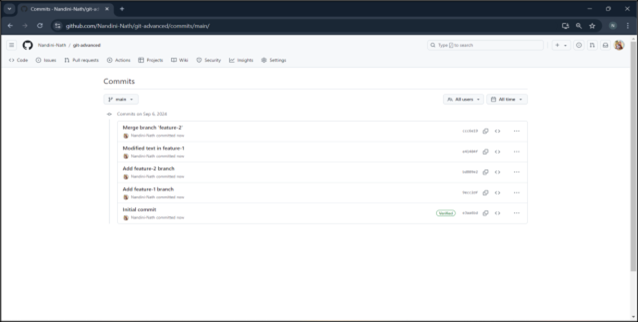
\includegraphics[width=0.8\linewidth]{LaTex_group_5/commit_history.png} % Adjusted width
     \hspace{4 cm}
    \caption{Screenshot of the GitHub repository showing the commit history.}
\end{figure}

% Screenshot 2 
\begin{figure}[h!]
    \centering
    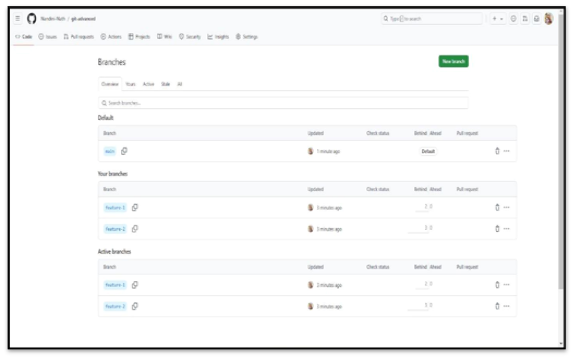
\includegraphics[width=0.8\linewidth]{LaTex_group_5/branching.png} % Adjusted width
     \hspace{4 cm}
    \caption{Screenshot of the GitHub repository showing the branching.}
\end{figure}
\newpage
\begin{tikzpicture}
    [remember picture, overlay]
    \draw[line width = 2pt, black] 
        ($(current page.north west) + (1cm,-1cm)$) 
        rectangle 
        ($(current page.south east) + (-1cm,1cm)$);
\end{tikzpicture}
\vspace{-1.5cm}
% Screenshot 3

\begin{figure}[h!]
    \centering
    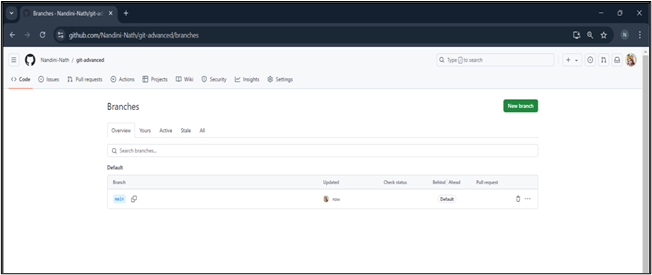
\includegraphics[width=0.8\linewidth]{LaTex_group_5/deleted_branches.png}
       \hspace{4 cm}
    \caption{Repository after deleting branches 'feature-1' and 'feature-2'.}
    \label{fig:enter-label}
\end{figure}
% Screenshot 4
\hspace{6 cm}
\begin{figure}[h!]
    \centering
    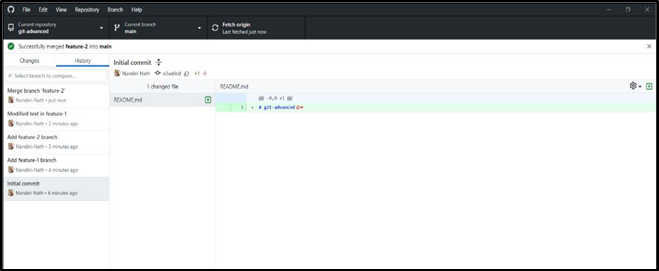
\includegraphics[width=0.8\linewidth]{LaTex_group_5/git_log.png} % Adjusted width
    \hspace{4 cm}
    \caption{Screenshot of the local machine showing the Git log.}
\end{figure}
\hspace{6 cm}
% Screenshot 5
\begin{figure}[h!]
    \centering
    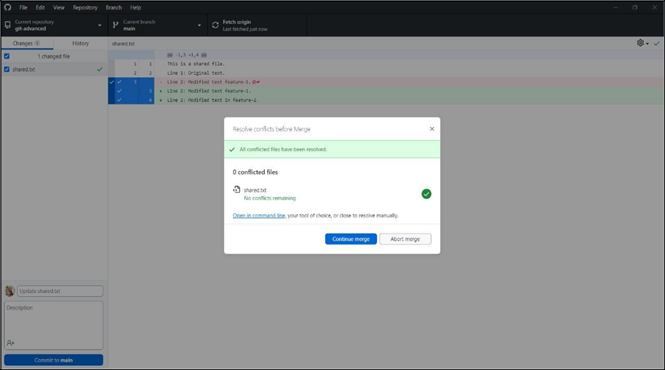
\includegraphics[width=0.8\linewidth]{LaTex_group_5/conflict_resolution.png} % Adjusted width
       \hspace{4 cm}
    \caption{Screenshot of the local machine showing conflict resolution.}
\end{figure}
\newpage
\begin{tikzpicture}
    [remember picture, overlay]
    \draw[line width = 2pt, black] 
        ($(current page.north west) + (1cm,-1cm)$) 
        rectangle 
        ($(current page.south east) + (-1cm,1cm)$);
\end{tikzpicture}
\vspace{-1.5cm}
\subsection*{\Huge{Write-Up: Experience with Git Branching and Merging}}
\\\
\paragraph {This assignment focused on the use of Git branching and merging to manage features in a collaborative environment. After creating separate branches for feature-1 and feature-2, each was developed independently.
When merging feature-1 into the main branch, there were no conflicts. However, the merge of feature-2 caused a conflict in the shared.txt file. Conflict resolution was done manually, ensuring that the changes from both branches were retained.
The practical experience highlighted the importance of clear commit messages and Git’s branching capabilities for parallel development and conflict management.}

\end{document}
